\UseRawInputEncoding
\documentclass{lab}

\usepackage{graphicx}
\usepackage{float}
\usepackage{soul}

\title{ENGG1003 - Lab 1}
\author{Brenton Schulz}
\date{\today}

\begin{document}
\maketitle

\section{Introduction}
This laboratory exposes you to the fundamental tools required to write computer programs in C. No prior programming experience is assumed but basic computer literacy is required. Advanced PC gaming skills such as:

\begin{itemize}
\item Editing .cfg or .ini files
\item Configuring command line arguments (eg: via a shortcut or Steam)
\item Debugging complicated driver problems
\item Using a game engine's debug console (typically accessed via the tilde \textasciitilde\ key)
\item Use of keyboard shortcuts
\item Hosting LAN parties and knowing how to configure the network
\end{itemize}

are also excellent preparation for your programming adventure. If you lack this experience then hopefully today's lab gets you up to speed.

The ENGG1003 labs involve sitting at a PC with 20 to 40 other students and working through lab exercises. Most weeks the lab exercises are there for you to learn, others there will be an assessment task which must be marked by a lab demonstrator before you leave.

The lab demonstrator's job is to answer questions you have about the material and help you work through unexpected problems. There will be limits to how much help they can provide during assessment tasks (default assumption is zero) but during non-assessed labs you can ask them anything you want.

Their job is not \textit{necessarily} to directly answer your question but to provide information which best supports your learning. This means that, instead of giving you an answer, they may guide you through the process of using Google/reference documentation/etc to help you become an independent learner.

While you are going through this course it is a near certainty that you will encounter difficult problems which take hours (or even days) to solve. This is normal. Engineering is \textit{hard} and watching other students solve problems faster than you is demoralising. Don't hesitate to ask for help. Talk to people and \st{copy from them}\footnote{Seriously, don't do this.} solve problems together. Don't suffer in silence.

\begin{figure}[H]
\begin{center}
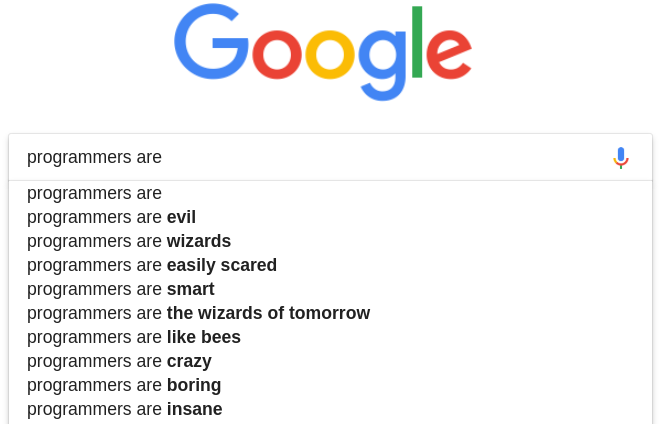
\includegraphics[width=0.6\textwidth]{Wk1Images/google.png}
\end{center}
\caption{This image isn't really relevant, I just thought it was funny. Yes, it is real.}
\end{figure}

\pagebreak
\tableofcontents

\pagebreak

\section{Software Installation}

This section of ENGG1003 introduces you to the ``C'' programming language. Before getting started you should check that the software below is installed on the PC you are using. Links are provided for installation on a personal computer. If you are using a university PC use the Software Center, documented below.

Software List:

\begin{itemize}
\item Code::Blocks - Download ``codeblocks-17.12mingw-setup.exe'' from \url{http://www.codeblocks.org/downloads/26}
\item Git for Windows - Download ``Git-2.25.1-32-bit.exe'' from \url{https://github.com/git-for-windows/git/releases/tag/v2.25.1.windows.1}
\end{itemize}

To find both packages on a lab PC:

\begin{itemize}
\item Code::Blocks - Search ``codeblocks'' in the Start menu and look for the result shown in Figure \ref{fig:codeblocksStart.png}.

\begin{figure}[H]
\begin{center}
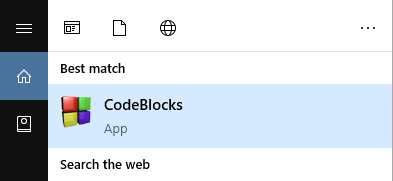
\includegraphics[width=0.4\textwidth]{Wk1Images/cbstart.png}
\end{center}
\caption{The Start menu search result for Code::Blocks.}
\label{fig:codeblocksStart}
\end{figure}

\item Git for Windows - There is no Start menu entry for this software, it is only accessed by right click'ing in a location in Windows Explorer.

Test for its installation by opening Windows Explorer (shortcut is windows button + E), navigating to \texttt{U:\textbackslash}, and right click somewhere. The menu which appears should list ``Git GUI Here'' and ``Git Bash Here'' as shown in Figure \ref{fig:gitforwindowsmenu}.

\begin{figure}[H]
\begin{center}
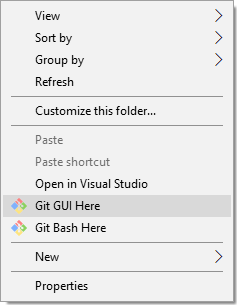
\includegraphics[width=0.4\textwidth]{Wk1Images/gitMenu.png}
\end{center}
\caption{Git for Windows is listed when right click'ing in (or on) a folder when browsing Windows Explorer.}
\label{fig:gitforwindowsmenu}
\end{figure}

\end{itemize}

In case software is not installed all university PCs contain a ``Software Center'' app which allows students to install software on university PCs from a university managed package repository.

To install software:

\begin{enumerate}
\item Use the Start menu to search for the Software Center as shown in Figure \ref{fig:SoftwareCenter}.

\begin{figure}[H]
\begin{center}
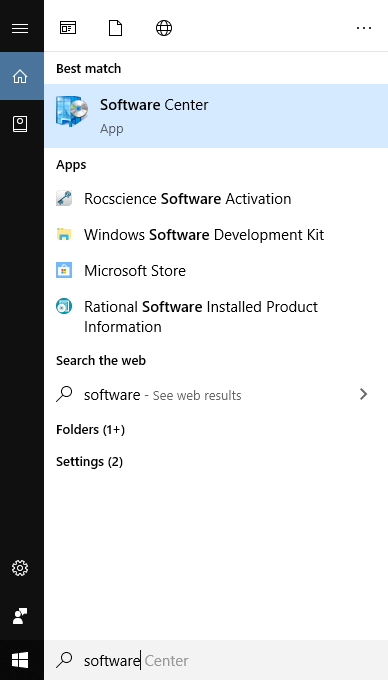
\includegraphics[width=0.4\textwidth]{Wk1Images/softwareSearch.png}
\end{center}
\caption{Use the Start menu to find the Software Center app.}
\label{fig:SoftwareCenter}
\end{figure}

\item After the Software Center opens, search for the package you need (In this case, either ``codeblocks'' or ``git for windows'') using the search bar in the top right as shown in Figure \ref{fig:SoftwareCenterGit}.

\begin{figure}[H]
\begin{center}
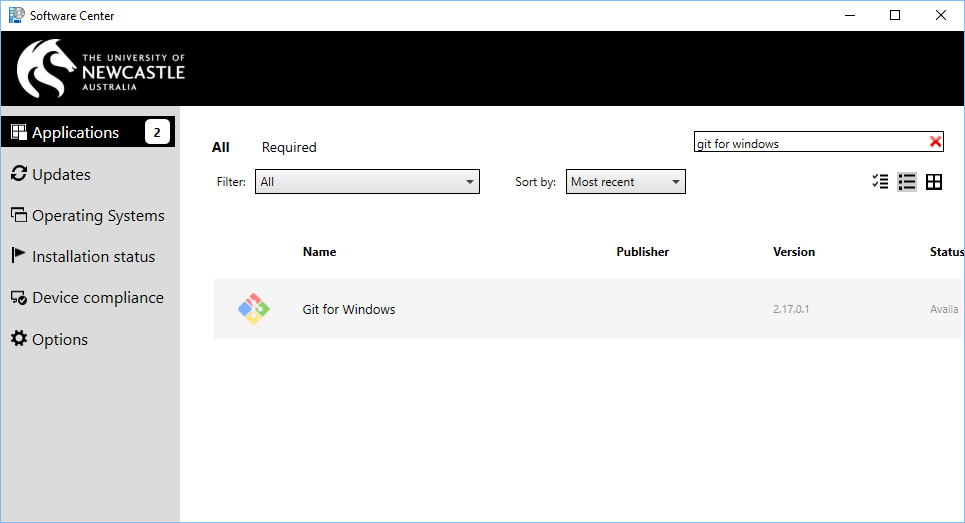
\includegraphics[width=0.9\textwidth]{Wk1Images/softwareSearchGit.PNG}
\end{center}
\caption{Searching for Git for Windows using the Software Center. Note that it is listed as ``available''; this implies that it is not installed.}
\label{fig:SoftwareCenterGit}
\end{figure}

\item Clicking a search result brings up some package information and an install button as shown in Figure \ref{fig:SoftwareCenterInstall}. Click the install button.

\begin{figure}[H]
\begin{center}
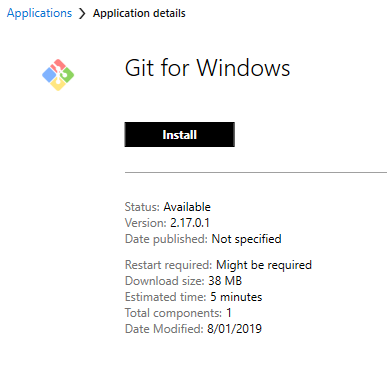
\includegraphics[width=0.6\textwidth]{Wk1Images/softwareInstall.PNG}
\end{center}
\caption{Click ``Install'' and wait a minute for the package to be installed.}
\label{fig:SoftwareCenterInstall}
\end{figure}

\end{enumerate}

\pagebreak
\section{C Programming Basics}
In order to write programs in C (and most other languages) the following software tools are required:

\begin{itemize}
\item An \textit{editor}, to create and edit raw text files.
\item A \textit{compiler}, to convert your text files into an \textit{executable} file.
\end{itemize}

A programming editor is very different to a \textit{word processor} (eg: Microsoft Word) in that it displays and stores raw ASCII text only. What you see printed to the screen represents the \textit{actual data} stored in the file. By contrast, Word will store a combination of text and display formatting and, as such, is not suitable for writing code.

Programming editors will generally have features optimised for coding, such as:

\begin{itemize}
\item Syntax highlighting
\item Line numbering
\item Auto completion
\item Pre-emptive error notifications
\item Communication with the compiler to highlight errors
\item Automatic indenting
\item Highlighting of matching blocks 
	\begin{itemize}
		\item ie: an easy method to find matching pairs of ( ), \{ \}, " ", etc.
	\end{itemize}
\end{itemize}

It is hoped that you will discover these features and learn to work with them. In time you will learn which features work well with your style and which simply get in the way.

For the time being the ``compiler'' noun will be used to colloquially reference a highly complex set of software tools which turn your source code into an executable binary file. You will be shielded from the details until otherwise necessary.

\pagebreak
\subsection{Introduction to Code::Blocks}

Code::Blocks is a relatively simple \textit{integrated development environment} (IDE). It contains a coding-oriented editor, build system which runs a pre-configured compiler, and debug interface. It is the recommended development environment for ENGG1003.

To open Code::Blocks and create a new ``hello world'' template project perform the following steps:

\begin{enumerate}
\item Find Code::Blocks in the Start menu and click it:

\begin{figure}[H]
\begin{center}
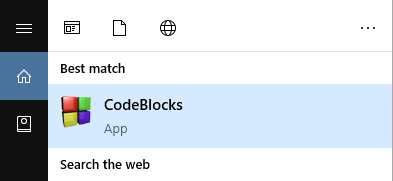
\includegraphics[width=0.6\textwidth]{Wk1Images/cbstart}
\end{center}
\end{figure}

\item Code::Blocks searches for installed compilers on startup. Make sure GNU GCC Compiler is detected and click OK.

\begin{figure}[H]
\begin{center}
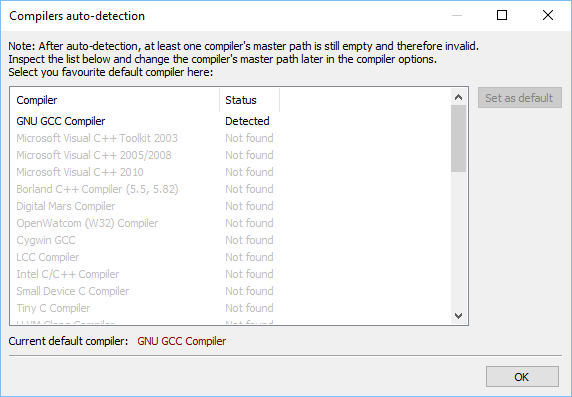
\includegraphics[width=0.6\textwidth]{Wk1Images/cb0.png}
\end{center}
\end{figure}

\item If this comes up make your own selection and click OK. I'd recommend the 3rd option so that clicking a \texttt{.c} file opens it in Code::Blocks.

\begin{figure}[H]
\begin{center}
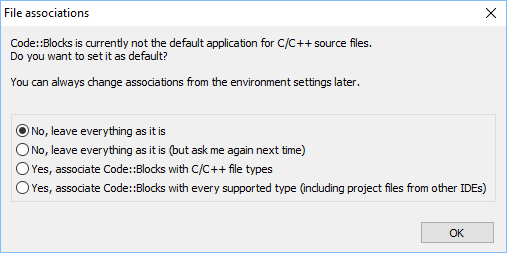
\includegraphics[width=0.6\textwidth]{Wk1Images/cb0b}
\end{center}
\end{figure}

\item After closing the previous dialogue box we are finally greeted by the main screen. It currently doesn't have a project open so there is no code to edit and no files listed in the ``Workspace'' (left side).

\begin{figure}[H]
\begin{center}
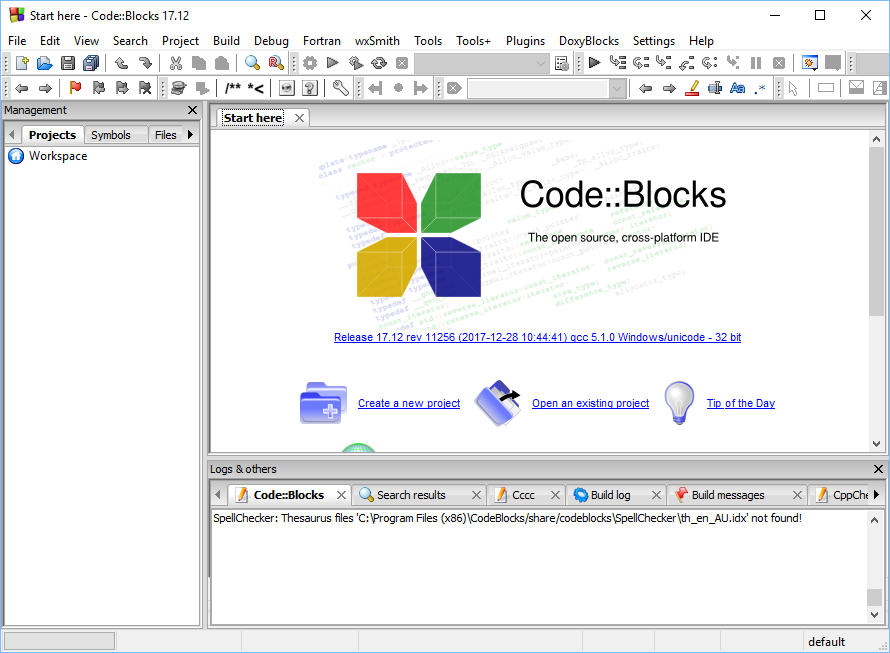
\includegraphics[width=0.8\textwidth]{Wk1Images/cb1}
\end{center}
\end{figure}

\item Create a new project by clicking File > New > Project...

\begin{figure}[H]
\begin{center}
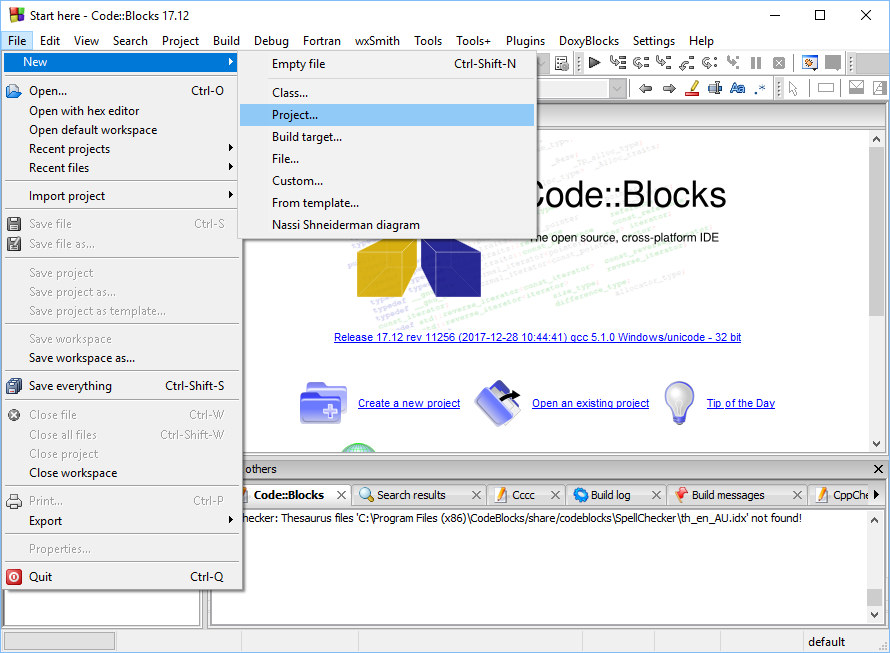
\includegraphics[width=0.8\textwidth]{Wk1Images/cb2}
\end{center}
\end{figure}
\pagebreak

\item Select ``Console application'' (middle left) and click ``Go'' (upper right).

\begin{figure}[H]
\begin{center}
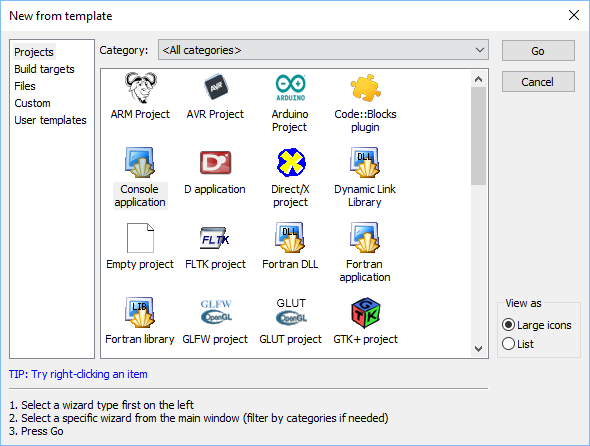
\includegraphics[width=0.8\textwidth]{Wk1Images/cb3}
\end{center}
\end{figure}

\item Select ``C'' in the middle list and click ``Next''

\begin{figure}[H]
\begin{center}
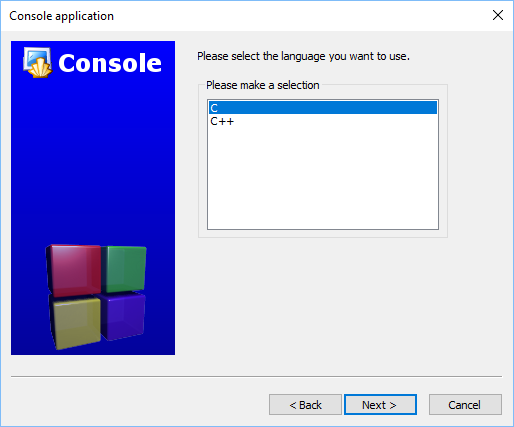
\includegraphics[width=0.8\textwidth]{Wk1Images/cb4}
\end{center}
\end{figure}

\pagebreak

\item Give your project a title and select a folder to store it by clicking the ``...'' button to the right of the ``Folder to create project in'' text box. I recommend storing it on \texttt{U:\textbackslash} as this is a network share mounted on any university PC when you log in. Later, we will use the version control software ``git'' and host our project files on the cloud service ``GitHub''.

Click ``Next'' when you are done.

\begin{figure}[H]
\begin{center}
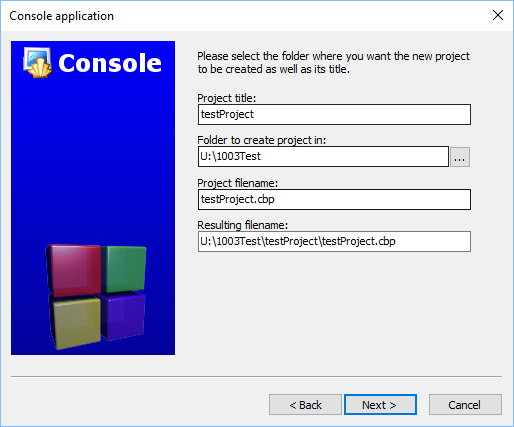
\includegraphics[width=0.8\textwidth]{Wk1Images/cb5}
\end{center}
\end{figure}

\item Don't change anything on this screen. Just click ``Finish''.

\begin{figure}[H]
\begin{center}
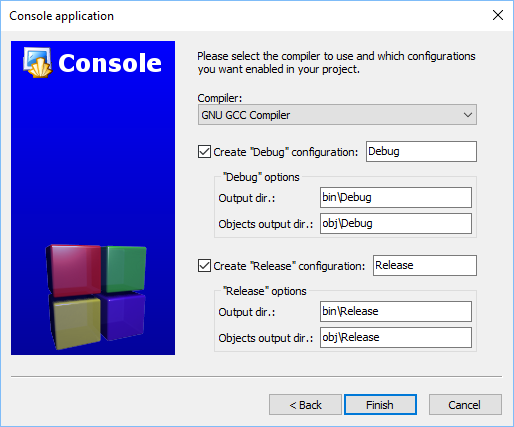
\includegraphics[width=0.6\textwidth]{Wk1Images/cb6}
\end{center}
\end{figure}

\item The project is now created and you should be seeing a screen similar to Figure \ref{fig:codeblocksTemplate}. Click the ``\texttt{+}'' symbol next to ``Sources'' to list the files in the project and double click ``main.c'' to make it appear in the editor window.

 The code listing in the main editor window is a classic ``hello world'' program For unknown historical cultural reasons printing ``Hello World!'' to the screen is the first thing everybody must learn when studying programming.

\item Compile and run the project by clicking the ``green play button and gear'' icon, highlighted by the professionally drawn blob of a red arrow in Figure \ref{fig:codeblocksTemplate}. This performs a ``build and run'' process. In this context ``build'' is just another word for ``compile''; the process of turning program code into a \textit{binary} that the computer can execute.

\begin{figure}[H]
\begin{center}
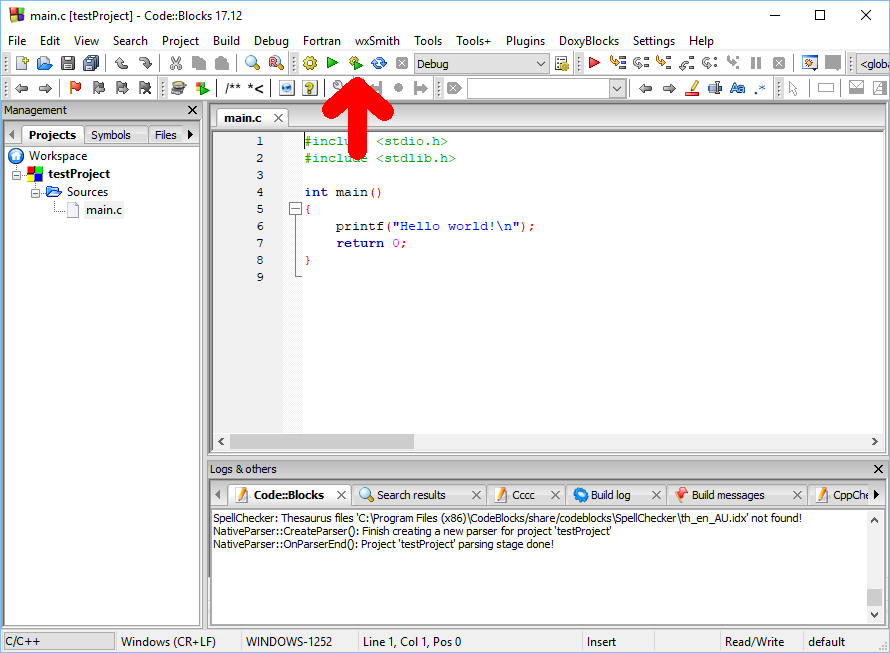
\includegraphics[width=0.8\textwidth]{Wk1Images/cb7}
\end{center}
\caption{The ``Hello World'' template project created by Code::Blocks.}
\label{fig:codeblocksTemplate}
\end{figure}
\pagebreak
\item If there are no errors (if there are ask a demonstrator for help) the Windows command prompt window shown in Figure \ref{fig:cmdcom} will appear. This is your program running in a console, the ``Hello world!'' text is visible at the top.

The ``Process returned 0...'' text relates to the \texttt{return 0;} at the bottom of the code listing. You don't need to worry about what this is now, we will study ``return values'' in later weeks. Suffice to say that if you see this everything worked.

\begin{figure}[H]
\begin{center}
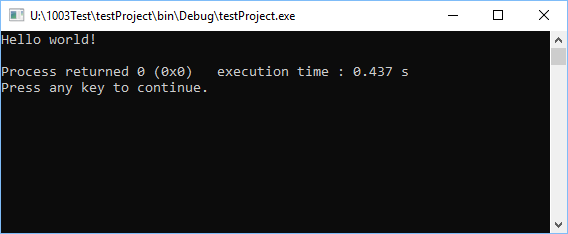
\includegraphics[width=0.8\textwidth]{Wk1Images/cb8}
\end{center}
\caption{}
\label{fig:cmdcom}
\end{figure}

\end{enumerate}
\pagebreak
\begin{task}{}{}

\begin{enumerate}

\item Running the default template demonstrates \textit{standard output}. Modify the code to match that in Listing~\ref{lst:stdio}.
\\ \\
\textbf{NB:} You can use either tabs or spaces for indenting. Tabs is fewer keystrokes, spaces are more well defined. Some editors change the width of a tab and this causes illogical anger in some programmers.
\\ \\
While making the changes you will observe Code::Blocks' auto-complete features. When, for example, you type a double quote " character it \textit{automatically} types two and places the cursor between them. The editor will also automatically indent new lines and provide auto-complete suggestions, although many of them will be inappropriate (it is, after all, just a computer program; not a science fiction grade artificial intelligence).

~\\
Also observe that when you write a \textit{function} name (eg: \texttt{scanf()}) you will be greeted with a pop-up which shows \texttt{int scanf(const chat*, ...)}. This is known as a \textit{function prototype} and is there to help you remember how a function is used. We will study this is more detail when functions are covered later in the semester.

~\\
What other ``helpful'' editor behaviour did you notice? Some of it will be annoying at first (some of it will be annoying \textit{forever}) but learning to work with the editor's features will improve your coding speed in the long term.

\begin{lstlisting}[style=CStyle,caption=A basic C program which demonstrates input and output.,label=lst:stdio]
#include <stdio.h>
#include <stdlib.h>

int main()
{
	int k;
	scanf("%d", &k);
	printf("You entered: %d\n", k);
	return 0;
}
\end{lstlisting}

\item After editing the code build and run it again. After it is compiled you will notice that the console is just displaying a \texttt{\_} cursor. This is because \texttt{scanf()} waits for data to be typed (specifically, it will wait until a new line character, ASCII value 10, is sent).

\item Type an integer and press \texttt{enter / return}.

\item After pressing enter the console should display the text ``\texttt{You entered: 123}''.

\item Run the program again except this time don't type just an integer, try typing a word, or a word containing a number, or a number followed by letters (with and without a space). What is the behaviour each time?

\end{enumerate}
\end{task}\label{tsk:stdio}


\pagebreak
\subsection{Introduction to OnlineGDB - Optional}

\textbf{NB:} OnlineGDB is not necessary but you may find it useful if you are forced to use a computer which lacks a C compiler.

OnlineGDB is a basic (\textit{very} basic) browser-based development environment for a variety of programming languages. It gives you access to an editor, a small amount of cloud storage, compiler, and standard input~/~output. It also contains a \textit{debugging} feature however for technical reasons\footnote{It only allows one debug session per IP address. The entire campus uses the same public IP so we can't use it in labs.} we won't be using it.

All compilation and execution is performed on the OnlineGDB server. As such, the service has an incredibly low barrier to entry: there is (almost) zero installation/configuration required to get started running code.

\begin{task}{}{}
\begin{enumerate}

\item Open a web browser and navigate to \url{http://www.onlinegdb.com}.

\item Configure OnlineGDB to run C code by selecting ``C'' from the ``Language'' drop-down box in the upper-right.
\end{enumerate}

This website supports many languages\footnote{MATLAB is not one of them because it is a \textit{very} expensive commercial package.} so feel free to come back here later if you're interested in learning any of the others. Python, although not taught in an Engineering degree, is a common choice for Engineering PhD students as a free MATLAB alternative and is probably worth playing around with.

\textbf{NB:} If a demonstrator sees you using Edge or IE they may instinctively think you need more help than students using Chrome or Firefox.
\end{task}

\begin{figure}[H]
\begin{center}
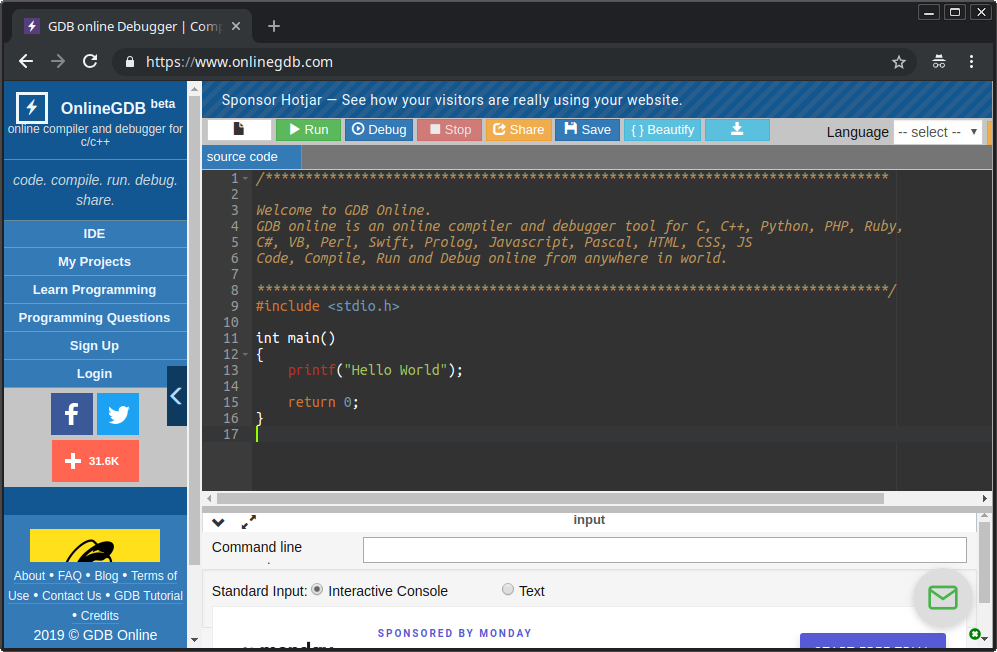
\includegraphics[width=\textwidth]{Wk1Images/onlinegdb.png}
\end{center}
\caption{The view when OnlineGDB is first opened.}\label{fig:onlinegdb}
\end{figure}

After OnlineGDB has loaded you will be greeted with the screen seen in Figure \ref{fig:onlinegdb}. The large area in the middle is the editor screen, this is where you will type C code. Immediately you can observe that this editor supports line numbering and syntax highlighting.

Above the editor is a toolbar which, from left to right, performs the following functions:

\begin{enumerate}
\item Create a blank new file
\item Run the project
\item Debug the project (not used in ENGG1003)
\item Stop execution of a running program
\item Share - Generates a link to your current source code
\item Save - When logged in this saves the project files to your personal cloud storage
\item \{ \} Beautify - Modifies your code's whitespace to adhere to the OnlineGDB indenting style (NB: I tried this at time of writing and it didn't work on my personal computer. Go figure.)
\item Download - Downloads the currently viewed file.
\end{enumerate}

The area below the editor is where standard output is written to and standard input read from. When the code is run its appearance changes to that of a basic console (ie: the GUI elements disappear and it becomes just text).

\begin{task}{}{}
\begin{enumerate}
\item Observe that there is already a template C listing in the editor.
\item Click the green Run button.
\end{enumerate}
The box at the bottom of the screen will produce a ``Compiling'' animation and, after execution of the template code, will produce the output seen in Figure \ref{fig:onlinegdb_hello}.
\end{task}

\begin{figure}[H]
\begin{center}
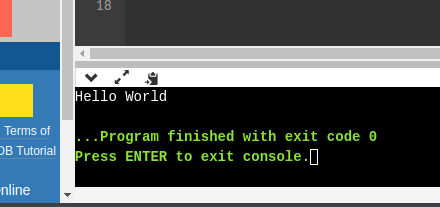
\includegraphics[width=0.7\textwidth]{Wk1Images/onlinegdb_hello.png}
\end{center}
\caption{A cropped screenshot showing the "Hello World" program output.}\label{fig:onlinegdb_hello}
\end{figure}

\textbf{Off-topic note:} Remember the ``returns zero to the operating system'' comment in lecture 1? Well that's what the text ``...Program finished with exit code 0'' is referencing. The 0 is the number that \texttt{main()} \textit{returned}. We will learn about \textit{function return values} later in the semester.

\pagebreak
\section{Compiler Errors and Warnings}

This section will demonstrate several common compiler \textit{errors} and \textit{warnings}.

An error occurs when the code does not meet the rigorous and unambiguous syntax rules specified in the ANSI C standard and, as such, the compiler does not know how to interpret the code. For example, if you miss a \texttt{"} symbol inside a \texttt{printf()} where does the text to be printed end? This can't be assumed because there are not enough rules about what you can and can't write in this context. As such, missing a \texttt{"} will produce a \textit{syntax error}.

By contrast, a warning occurs when the code is in some way ``mildly'' problematic but the compiler is still able to make assumptions about what the code should do and produce a binary executable. For example, if the \texttt{return 0;} at the end of \texttt{main()} is missing the compiler will throw it in for you because, well, what else is it going to do at the end of \texttt{main()}?\footnote{The programmer could want \texttt{main()} to return a value other than zero but it is overwhelmingly common to just return zero here. Historically, a program returning zero means ``the program finished without error'' and non-zero indicates some kind of error code.}

Unfortunately compiler errors can be \textit{highly} technical and difficult to interpret. Furthermore, they often report an error on a line \textit{after} the actual mistake! The exercises below will give you some experience with interpreting compiler errors but this is a topic in which you will likely engage in ``life-long learning''.

\subsection{Missing a semicolon}

\begin{task}{}{}
\begin{enumerate}
	\item If you have not done so already, get the code shown in Listing \ref{lst:stdio} working correctly.
	\item Remove the semicolon (the ; character) from the end of line 6.
	\item Compile the code, what error did the compiler produce? Which line is the error is on?
\end{enumerate}
\end{task}
	
	The compiler errors in Code::Blocks will look something like Listing \ref{lst:errs}, but formatted better.
	
	\begin{lstlisting}[caption=The multiple errors produced by removing a \textit{single} semicolon.,label=lst:errs,basicstyle=\ttfamily\small,frame=single]
||=== Build: Debug in testProject (compiler: GNU GCC Compiler) ===|
U:\1003Test\testProject\main.c||In function 'main':|
U:\1003Test\testProject\main.c|7|error: expected '=', ',', ';', 'asm' or
     '__attribute__' before 'scanf'|
U:\1003Test\testProject\main.c|7|error: 'k' undeclared (first use in this function)|
U:\1003Test\testProject\main.c|7|note: each undeclared identifier is reported only
     once for each function it appears in|
||=== Build failed: 2 error(s), 0 warning(s) (0 minute(s), 0 second(s)) ===||
	\end{lstlisting}

The first error (\texttt{error: expected '=' , ‘,’, ‘;’, ‘asm'}... etc.) is telling you that something was missing and the compiler noticed the omission at line 7. In this case we removed a ; so that's what is missing. Note, however, that while the error was reported to be on line 7 the omission was actually on line 6! Also observe the extra technical jargon that you don't understand yet (what is \textit{\_\_attribute\_\_}??). Some of these are, in fact, beyond the scope of ENGG1003. You have to get used to reading text you don't understand and extracting the small pieces of information you actually need.

Let's look at the second error: \texttt{'k' undeclared}. Wait, wasn't \texttt{int k} still in our source code? Why is the compiler complaining that it is undeclared when it is \textit{right there}? The problem is that by removing the semicolon the declaration syntax was incorrect, so the compiler did not interpret that line as a declaration. It didn't find the expected ; threw its hand in the air and gave up.

The final line (\texttt{each undeclared identifier...} etc.) is just telling you that if you forget to declare a variable the compiler will only tell you about it \textit{once}. This is because it could appear multiple times and producing the same error over and over is redundant and confusing.

Lets try a different syntax error.

\subsection{Missing a Quote Symbol}

\begin{task}{}{}
\begin{enumerate}
\item Fix the previous error by re-inserting the semicolon.
\item Remove the closing " from the \texttt{printf} line so it reads:
\begin{lstlisting}[style=CStyle]
printf("You entered: %d\n, k);
\end{lstlisting}
\end{enumerate}
\end{task}

You will see an immediate change to the syntax highlighting; all characters between where the " was and the end of the line are now blue\footnote{Yeah, I know that these notes use different syntax highlighting colours to Code::Blocks. Sorry, fixing is on my TODO list for 2021.} in the Code::Blocks editor, as if they were still inside the double quotes. Take-home message: \textit{pay attention to syntax highlighting!}

Again, removing a \textit{single character} generated a slew of errors:

\begin{lstlisting}[basicstyle=\ttfamily,caption=Errors produced by removing a \texttt{"} character.,frame=single]
||=== Build: Debug in testProject (compiler: GNU GCC Compiler) ===|
U:\1003Test\testProject\main.c||In function 'main':|
U:\1003Test\testProject\main.c|8|warning: missing terminating " character|
U:\1003Test\testProject\main.c|8|error: missing terminating " character|
U:\1003Test\testProject\main.c|9|error: expected expression before 'return'|
U:\1003Test\testProject\main.c|10|error: expected ';' before '}' token|
||=== Build failed: 3 error(s), 1 warning(s) (0 minute(s), 0 second(s)) ===|
\end{lstlisting}

Observe how missing the closing " generates both an error and a warning at different locations. Why does it do this? To be honest, I don't know; I've only been using gcc for 20 years, there's always \textit{something} that you haven't learned yet. In the end it doesn't matter, an error exists that needs to be fixed before the compiler can output an executable.

Missing the " generated two other errors as without the " the \texttt{printf} \textit{expression} was not completed. In C an expression can be thought of as ``a syntactically complete line of code that does something unambiguous''. This is a \textit{very} informal definition but it will do for now. In order to complete the \texttt{printf} expression the syntax rules require the closing ", a closing right parenthesis ) [to match the opening left parenthesis (] and a semicolon ;. Removing the " character makes the compiler think that the existing ``\texttt{);}'' string at the end of the line is actually part of the data to be printed, not part of the C expression syntax (as such, the expression was never finished, leaving the compiler with an unresolved tension that will stay with it \textit{all day}\footnote{\url{https://xkcd.com/859/}}.

Remember how missing a ; caused errors on lines \textit{below} where the error actually was? Well the same thing has happened here. Because the \texttt{printf()} line was malformed an error occurred on the line below it (\texttt{expected expression before return}) \textit{and} the one below that (\texttt{expected ; before \} token}); C can be incredibly unforgiving!

\pagebreak

\subsection{Failing to Define \texttt{main()}'s Return Type}

Enough about errors, the final example in this section demonstrates a compiler \textit{warning}. 

\begin{task}{}{}
\begin{enumerate}
\item Fix the previous error by re-inserting the appropriate quote symbol.
\item Remove \texttt{int} before \texttt{main} Listing \ref{lst:warn}

\begin{lstlisting}[style=CStyle,caption=Example code which generates a warning.,label=lst:warn]
main()
{
    int k;
    scanf("%d", &k);
    printf("You entered: %d\n", k);
    return 0;
}
\end{lstlisting}
\end{enumerate}
\end{task}

Compiling this code generates the following compiler warning:

\begin{lstlisting}[basicstyle=\ttfamily,frame=single,caption=Compiler output produced when \texttt{main()} return type is omitted.,captionpos=b]
warning: return type defaults to ‘int’ [-Wimplicit-int]
\end{lstlisting}

Observe the warning printed to both the ``Build log'' and ``Build messages'' tabs towards the bottom of the Code::Blocks window.

The keyword which goes before \texttt{main()} specifies its \textit{return type}. This is the type of data which it sends back to the operating system on program exit. We will study function return types in later weeks. To my knowledge, operating systems only support the \texttt{int} return type (ie: an integer) so if you leave it out the compiler can quite safely \textit{assume} that's what should be there and only issue a warning instead of an error.

Generally speaking, warnings should be fixed when you see them. With experience you will know when they \textit{need} to be fixed (because the compiler is assuming something incorrectly) and when they can be ignored (because you have more important stuff to fix first).

No doubt you will see \textit{many} other errors and warnings during your foray into C programming. I still occasionally see new ones! If in doubt, throw the compiler output into Google, chances are someone on Stack Overflow\footnote{Why are you even taking this course? Stack Overflow is all you \textit{really} need, right?} has written a good explanation about it.

\pagebreak
\section{Comments}

So far all the code examples have been very basic and (hopefully) easy enough to read. In ``real'' projects, however, this is rarely the case and the code needs some kind of explanation for the reader to quickly, and accurately, understand what it does\footnote{Despite what you might believe experienced engineers and programmers are not wizards, our understanding is not \textit{magic}, it is based on experience and frequently needs supplementing with code comments.}.

You will hopefully gain experience with code comments as you progress through this course (and the rest of you career!) but for now we will just see the basics. Any text in the source files\footnote{Did I forget to define what source code, or source files, are? It is just another word for any programming code. It can also be called a source \textit{listing}.} which:

\begin{itemize}
\item Is between \texttt{/*} and \texttt{*/}, or
\item Is between \texttt{//} and the end of the line
\end{itemize}

is \textit{totally ignored} by the compiler and called a ``comment''.

Code comments are a place for you to explain how your code works, or what it does, to future people who work with it. It is also a great place to leave little memos to yourself, typically in the form of:

\texttt{// TODO: Fix this because <reasons>}.

In fact some code editors (like the Linux editor \texttt{vim}) will automatically highlight the text \texttt{TODO} so it is easy to find.

\begin{task}{}{} Take whatever source code is currently shown in Code::Blocks and add some comments in various places. Compile the code and observe that they have no effect.
\end{task}

Students frequently ask what should and should not be commented. In this course your comments should be written such that a student who is on track to achieve 50\% can understand what your code does without having to consult external reference material. This will seem overly verbose but it will be used in lieu of a better standard. As a general rule: if you needed to look up something in a reference manual when writing the code write a comment explaining it. For example:

\begin{lstlisting}[style=CStyle]
printf("%d\n", x); // %d formats an integer
\end{lstlisting}

Anything which, at first glance, appears to be at least a little bit cryptic should probably get a comment.

\pagebreak
\subsection{Intrinsic Documentation}

As a supplement to comments, \textit{intrinsic documentation} is the idea behind choosing informative names for variables and functions\footnote{No, you don't need to know what a function is yet. It is in week 5 or so.}. Compare, for example, the following two code listings:

\begin{lstlisting}[style=CStyle]
int main()
{
	float x, y;
	scanf("%f", &x);
	y = x*9.0/5.0 + 32.0;
	printf("%f\n", y);
}
\end{lstlisting}

\begin{lstlisting}[style=CStyle]
int main()
{
	float tempFahrenheit, tempCelcius;
	scanf("%f", &tempCelcius);
	tempFahrenheit = tempCelcius*9.0/5.0 + 32.0;
	printf("%f\n", tempFahrenheit);
}
\end{lstlisting}

The first one, especially without comments, is cryptic and not possible to understand without more information. The second, even if you don't understand all the code, quite intuitively converts Celcius to Fahrenheit.

You will observe that my notes break intrinsic documentation rules all the time. Sorry about that (the examples in notes will also tend to not do anything particularly useful, so it gets difficult when you try to document ``nothing'').

\pagebreak
\section{Basic Arithmetic in C}

So, it is Page \thepage{} of these notes and we haven't done anything \textit{useful} yet! Ok \textit{fine}, lets do some data processing.

In this section we will do some basic arithmetic on numbers which are read from the console (ie: read from \texttt{stdin}). Since we haven't learnt much C (or even much programming in general) these examples are either going to be a bit boring (because they don't do much) or look like black magic (because you haven't learned how they work yet). I have to ask you just to go through the motions at this stage. Hopefully exposure to the code below now will make it easier to understand how it works in the coming weeks.

Lets start with the basic C arithmetic operators:

\begin{table}[H]
\centering
\begin{tabular}{|l|c|}
\hline
Operation      & C Symbol \\
\hline
Addition       & +        \\
Subtraction    & -        \\
Multiplication & *        \\
Division       & /       \\
\hline
\end{tabular}
\caption{Basic arithmetic operators in C}
\end{table}

These are all \textit{binary} operators, meaning they operate on two \textit{operands}\footnote{An operand is one of the ``things'' that a mathematical operator operates on. Eg: In a + b the variables a and b are operands.}. This may feel obvious, but C includes several \textit{unary} operators and even a \textit{ternary} one (that nobody uses because it's confusing). Each operand could be a variable (eg: \texttt{a + b}), a constant (eg: \texttt{a + 5}) or some complicated expression (eg: \texttt{(2*a + 6) / (12 + b - x)} )\footnote{I contemplated leaving this closing parenthesis out to give you unresolved tension but I'm not quite \textit{that} evil.}.

We begin with a basic example:

\begin{task}{}{}
Modify your code to match that of Listing \ref{lst:arithmetic1}.

\begin{lstlisting}[style=CStyle,caption=A basic arithmetic example,label=lst:arithmetic1]
#include <stdio.h>

int main() {
	int k;
	printf("Enter an integer: ");
	scanf("%d", &k);
	k = 2*k;
	printf("That integer doubled is: %d\n", k);
	return 0;
}
\end{lstlisting}
\end{task}

Notice that this code has a \textit{slightly} improved user experience to previous examples; it produces a prompt (\texttt{Enter an integer: }) which tells you what to do. Also notice that the first \texttt{printf()} does \textit{not} end with a \texttt{\textbackslash n} (newline), so the number you type appears on the same line as the prompt.

The line \texttt{k = 2*k} takes the value of \texttt{k}, multiplies it by 2, then assigns that result back into the variable \texttt{k}. This is a \textit{crucial} concept in programming: the \texttt{=} symbol is \textbf{not} equality, \texttt{k = 2*k} is \textbf{not} an equation, it is \textit{assignment}. Assignment takes what's on the right, evaluates it, then stores it into the variable on the left.

\subsection{Operator Precedence Basics}

Just like in ``normal'' algebra different operators take precedence over others (PEMDAS / BODMAS anyone? How about those Facebook posts where \textit{everybody} gets this wrong?). You can view the full C operator precedence here: \url{https://en.cppreference.com/w/c/language/operator_precedence} but you don't need to learn all of it now, it will be covered more in future lectures.

For now we will observe some basic examples and look at how engineers can deal with the complexity of full C operator precedence.

The predominant engineer's approach to this topic is to vaguely learn how the language behaves and then throw parentheses everywhere just to be \textit{absolutely sure} that the intention is not ambiguous. In the end it is \textit{other people} who will have trouble reading your code, not the compiler, so you might as well make their job easy.

\begin{task}{}{}
Using the template in Listing \ref{lst:arithmetic2} implement the following equation in C:

\begin{equation}\label{eq:fraction}
y = 2x+3\times5.
\end{equation}

Remember that \texttt{*} is the multiplication operator in C and that a \texttt{;} is needed at the end of the line.


\begin{lstlisting}[style=CStyle,caption=A basic arithmetic example,label=lst:arithmetic2]
#include <stdio.h>

int main() {
	float x;
	float y;
	printf("Enter a number: ");
	scanf("%f", &x); // Note change of %d to %f
	// Complete the y = line below
	y = 
	printf("y: %f\n", y);
	return 0;
}
\end{lstlisting}
\end{task}

You will notice a few new things about Listing \ref{lst:arithmetic2}. Firstly, it uses the \texttt{float} datatype. This type will store any real number with a magnitude of $1.2 \times 10^{-38}$ to $3.4 \times 10^{38}$ with a precision of approximately 6 decimal digits. Its bigger brother, the \texttt{double} will be seen later.

The other major change is that inside \texttt{scanf} and \texttt{printf} the \texttt{\%d} has changed to \texttt{\%f}. The \texttt{f} stands for floating point, which is a standard method\footnote{The other major standard is known as \textit{fixed point}. Details are beyond ENGG1003 but you'll probably see it if you study enough digital signal processing (DSP).} for storing fractional numbers using only binary integers. The details are beyond this course, but you can read the details on Wikipedia: \url{https://en.wikipedia.org/wiki/IEEE_754}.

Back to the task at hand, have a go at implementing Equation \ref{eq:fraction} and see if the result works. Observe that you don't need to force precedence with parentheses because, in C, the multiplication operations are performed before addition.

\pagebreak

\begin{task}{}{}
Implement the following equations on line 8. What happens when you choose x to force a division by zero?

\begin{enumerate}
\item $y = 9x + 32$
\item $y = \frac{x}{1 - x}$.  This one will require parentheses.
\item $y = x^2 + 2x$. \textbf{NB:} C does \textit{not} include an exponent operator. Implement $x^2$ as \texttt{x*x}:
\item $y = \frac{x + 2}{x - 1}$
\end{enumerate}
\end{task}
\pagebreak
\section{A Very Brief Introduction to Git}

\textit{NB: Git is not in the course outline so it isn't strictly required nor assessed. It is, however, incredibly useful and included here because several 3rd and 4th year course coordinators (and industry contacts) asked me to expose you to it. I agreed.}

\textit{\textbf{NB 2:} github.com does not work on personal laptops when using campus wifi. A support ticket has been submitted to IT. It works on lab PCs and via 4G hotspotting. Also note that github's registration emails are dropped by the university's spam rules so you will need to sign up with a personal email address.}

Programming projects typically involve two potentially problematic issues:

\begin{enumerate}
	\item Multiple people contribute to the same project. How should their changes be ``merged'' into some kind of ``master'' source listing?
	\item Programmers frequently want to ``roll-back'' to an earlier code version.
\end{enumerate}

The second item arises from the fact that after going down a problematic design pathway it is typically much faster to scrap the idea and start again than it is to try and fix all the problems you just created. The fastest way to do this is to load up known-working code from the past and go from there.

As such, programmers designed so-called \textit{versioning} subsystems. These are ways of storing data which allows someone to access either a current or past version of a set of data.

In this course it will be \textit{recommended} that you take advantage of the modern versioning system known as Git. It was developed for tracking code in the Linux kernel and has since expanded to be an industry standard; even Microsoft purchased the website GitHub because it was \textit{just better} than anything else they had developed internally. I am using Git for tracking changes while writing course content and the Git host GitHub is also doubling as cloud storage as I move writing between three different computers.

The Git package can be installed on any computer, it doesn't even require a server / client architecture spread across two or more computers. GitHub is simply a website which hosts Git servers.

\begin{task}{}{} Navigate to:\\ \url{https://github.com/bschulznewy/engg1003/blob/master/Labs/LabWk1.pdf}
\\ \\ 
This is the GitHub ``repository'' that I have been using when writing ENGG1003 content. In particular, it is the Github copy of these lab notes.
\end{task}

The link is for a PDF document and you will see that GitHub automatically renders it inside the website. It will attempt to display any file directly linked to.

But that's not what we're here for. I want to show you the real power of Git: version tracking. Click on the ``History'' button to the top right of the PDF preview. You will be greeted with a view similar to that shown in Figure \ref{fig:githistory}. It lists the git \textit{commits} made which affect that file. A commit is a snapshot of what the entire repository looked like at a particular point in time. Each commit happens manually (ie: I type a command to cause a commit to be created) and is attached to a ``commit message'' which (hopefully) describes the changes which were made.

\begin{figure}[H]
\begin{center}
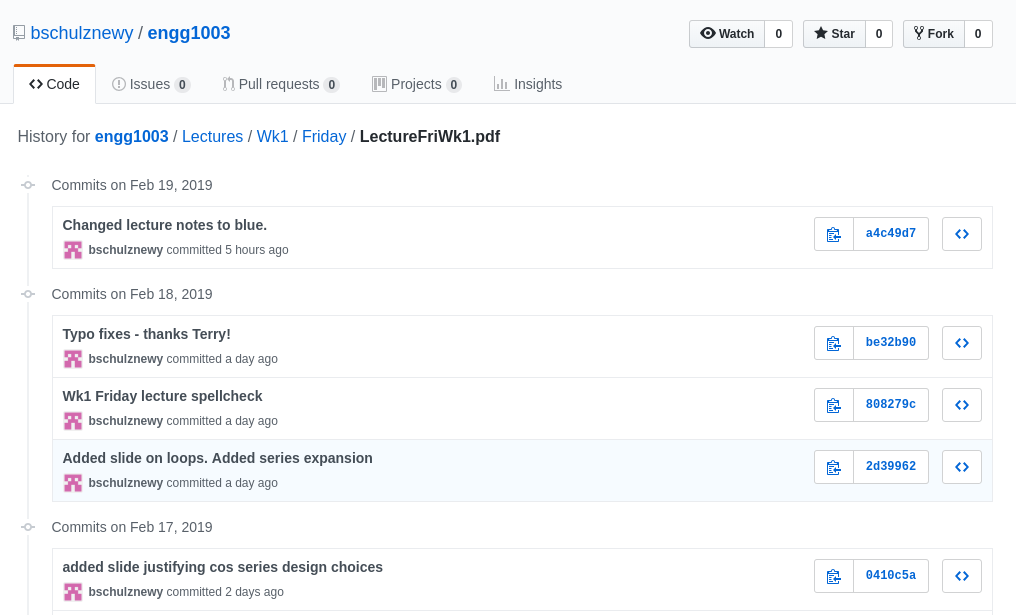
\includegraphics[width=0.8\textwidth]{Wk1Images/github_lecture.png}
\end{center}
\caption{The git repo history for the Friday lecture notes as it was last year - It will look very different now!.}\label{fig:githistory}
\end{figure}

If you click on a commit message you will see what changed in this particular git commit. An example is shown in Figure \ref{fig:gitchanges}.

\begin{figure}[H]
\begin{center}
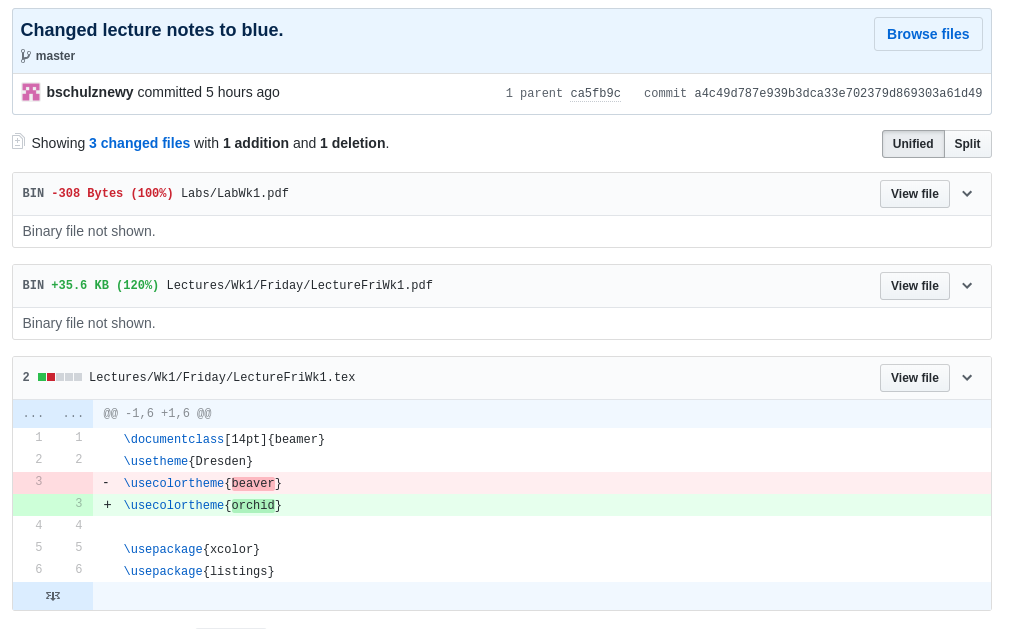
\includegraphics[width=0.9\textwidth]{Wk1Images/github_lecture_changes.png}
\end{center}
\caption{The changes which occured in a particular commit.}\label{fig:gitchanges}
\end{figure}

The box at the bottom of Figure \ref{fig:gitchanges} shows the actual changes which occurred. In this case I changed the colour theme for the lecture notes to roughly match that of the first lecture. The changes to the PDF are not shown because they would be unintelligible garbage (it is a binary file, not text).

Browse through the other recent commits \underline{\href{https://github.com/bschulznewy/engg1003/commits/master}{here}} and browse a few commits.

\begin{task}{}{} Go to \url{www.github.com} and create a GitHub account. You can use it to store all your code from this course (and other courses!). This allows advanced version tracking and cloud storage from the same service.\\
~\\
It has been reported that github.com currently (Feb 25th 2020) does not work through campus wifi when using a student account for wifi authentication. You can use a lab PC, your own computer through a 4G hotspot, or complete this section at home. A support ticket has been opened with campus IT.\\
~\\
The student email spam filter blocks the account activation emails from Github. \textbf{You will need to use a different email address to sign up!} This issue has also been lodged with IT.
\end{task}

\begin{task}{}{}
Use your new GitHub account to create a new Git repository and upload today's work to it using Git for Windows.

\begin{enumerate}

\item Open Windows Explorer (windows button + E) and navigate to the folder \textit{above} where your lab 1 code is stored.

\item Right click in this folder and select ``Git GUI here''.

\begin{figure}[H]
\begin{center}
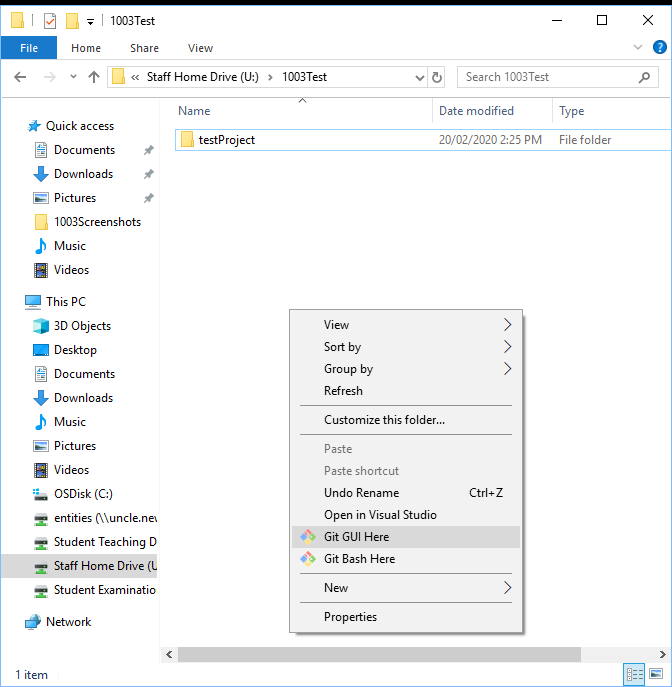
\includegraphics[width=0.9\textwidth]{Wk1Images/git1}
\end{center}
\end{figure}

\pagebreak
\item The dialog box shown in Figure \ref{fig:gitguicreate} appears. Click ``Create New Repository''.

\begin{figure}[H]
\begin{center}
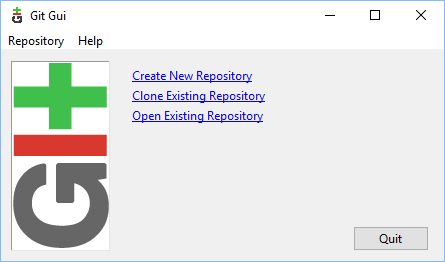
\includegraphics[width=0.7\textwidth]{Wk1Images/git2}
\end{center}
\caption{}
\label{fig:gitguicreate}
\end{figure}

\item You are then greeted with this dialogue box:

\begin{figure}[H]
\begin{center}
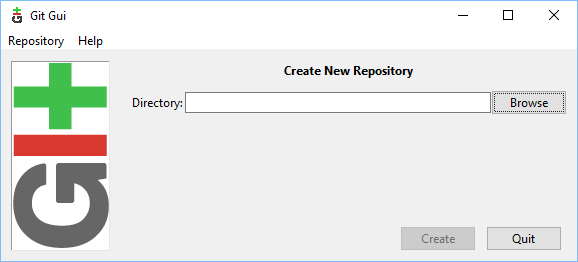
\includegraphics[width=0.7\textwidth]{Wk1Images/git3}
\end{center}
\end{figure}

\item Click ``Browse'' and select the folder which hold your lab 1 code:

\begin{figure}[H]
\begin{center}
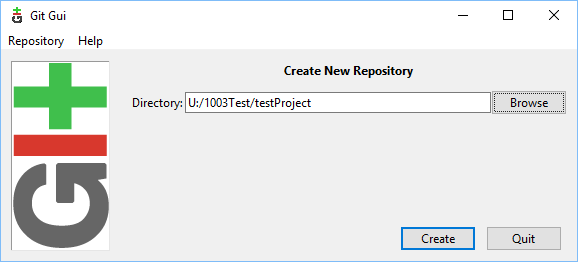
\includegraphics[width=0.7\textwidth]{Wk1Images/git4}
\end{center}
\end{figure}

\pagebreak

\item The main Git for Windows window should now appear:

\begin{figure}[H]
\begin{center}
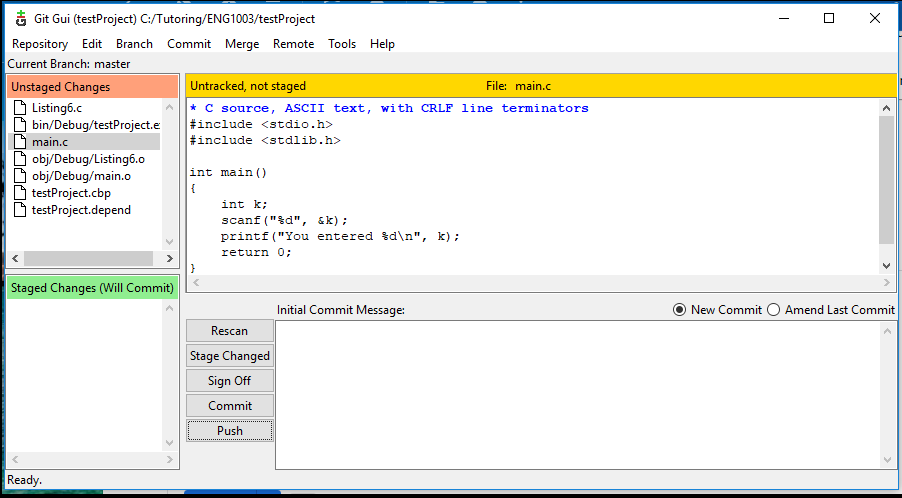
\includegraphics[width=0.7\textwidth]{Wk1Images/gitMainWindow}
\end{center}
\end{figure}

\item The ``Unstaged Changes'' section shows every file which has changed since the last \textit{commit} (snapshot of your work). Clicking on an unstaged change brings up a (potentially cryptic) view of the file in question showing what has changed. To create a commit and start the process of uploading it to Github:

\begin{enumerate}
	\item Click ``Stage Changed''
	\item Type a commit message in the bottom right. It should describe what has changed so you can easily find this commit later. For now you can type something like ``Initial commit''.
	\item Click ``Commit''
	\item Click ``Push''
	\item A new dialogue box will appear, we will come back to it later.
\end{enumerate}

\item Now navigate to \url{https://github.com} in a web browser, log in if necessary, and click the green ``New'' button:

\begin{figure}[H]
\begin{center}
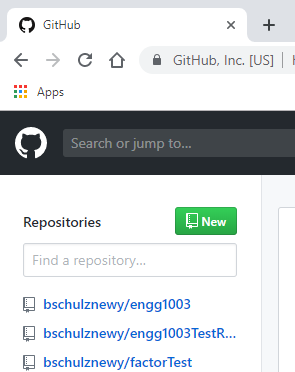
\includegraphics[width=0.5\textwidth]{Wk1Images/git5a}
\end{center}
\end{figure}

\pagebreak

\item Give the new repository a name and click the green ``Create repository'' button a the bottom:

\begin{figure}[H]
\begin{center}
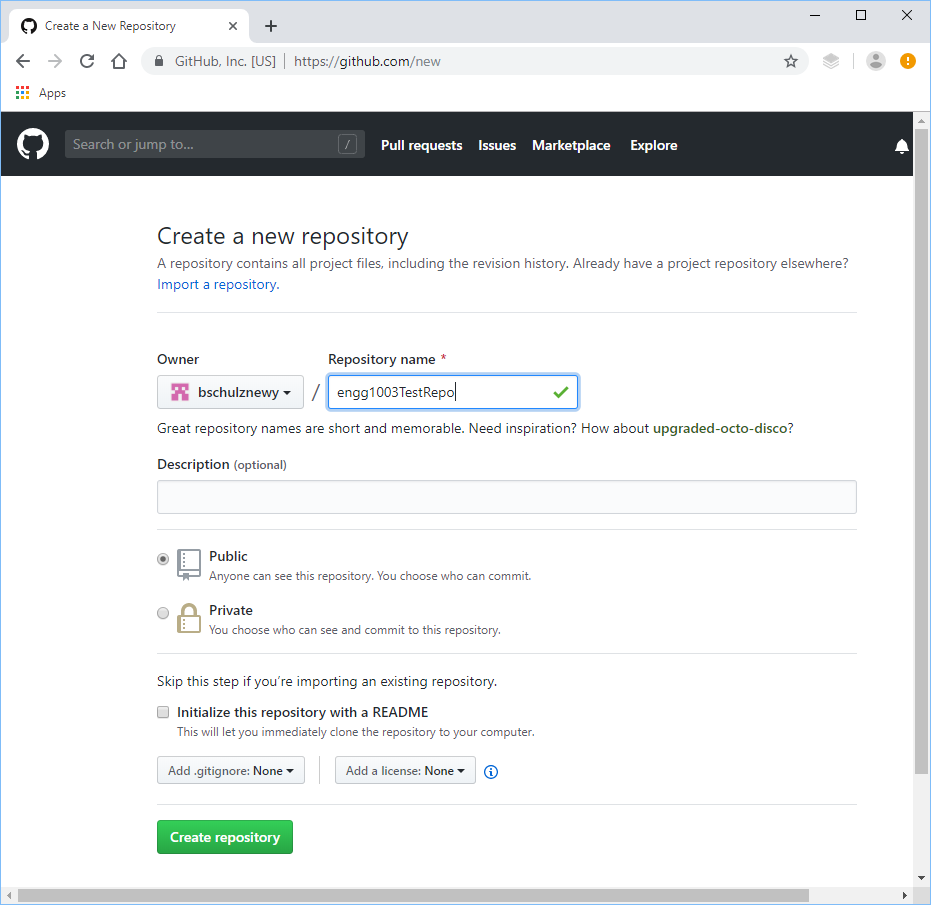
\includegraphics[width=0.9\textwidth]{Wk1Images/git5}
\end{center}
\end{figure}

\item In the ``Quick setup'' section ensure that the ``HTTPS'' button is selected and copy the URL in the text box next to it:

\begin{figure}[H]
\begin{center}
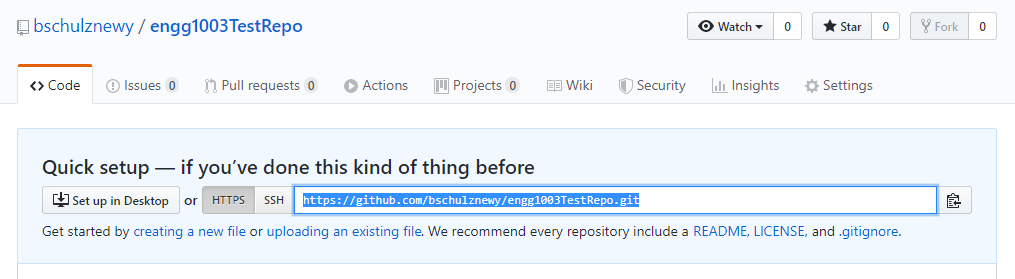
\includegraphics[width=0.9\textwidth]{Wk1Images/git6}
\end{center}
\end{figure}

\pagebreak

\item Back to Git for Windows, paste this URL in the text box next to ``Arbitrary Location:''

\begin{figure}[H]
\begin{center}
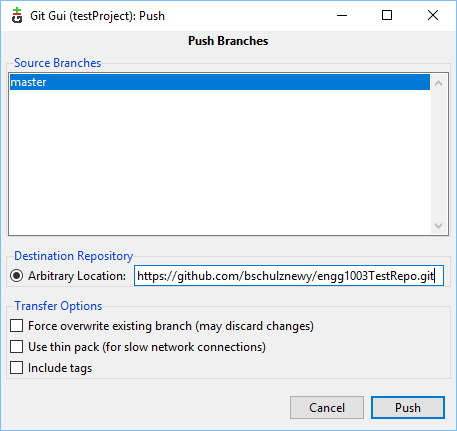
\includegraphics[width=0.6\textwidth]{Wk1Images/git7}
\end{center}
\end{figure}

\item In the dialogue box shown above, press ``Push''. This attempts to make a remote (``in the cloud'') copy of you repository at the URL you supplied.

\item Since the URL is on GitHub, the following login window appears. Type in your GitHub login details and click ``Login'':

\begin{figure}[H]
\begin{center}
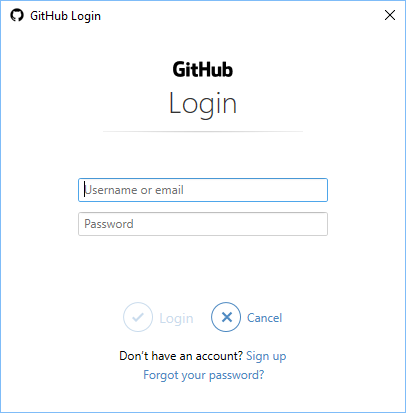
\includegraphics[width=0.6\textwidth]{Wk1Images/git8}
\end{center}
\end{figure}

\pagebreak

\item If your login is correct the window below will appear. The text output shows the progress of the upload (in Git language the ``Push'' operation).

\begin{figure}[H]
\begin{center}
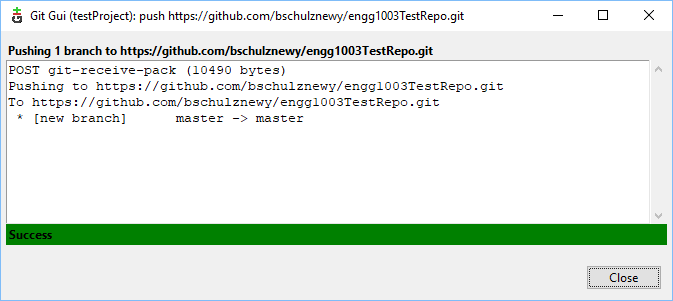
\includegraphics[width=0.9\textwidth]{Wk1Images/git9}
\end{center}
\end{figure}

\item If you navigate to the new repository on GitHub you will now see all the project files listed:

\begin{figure}[H]
\begin{center}
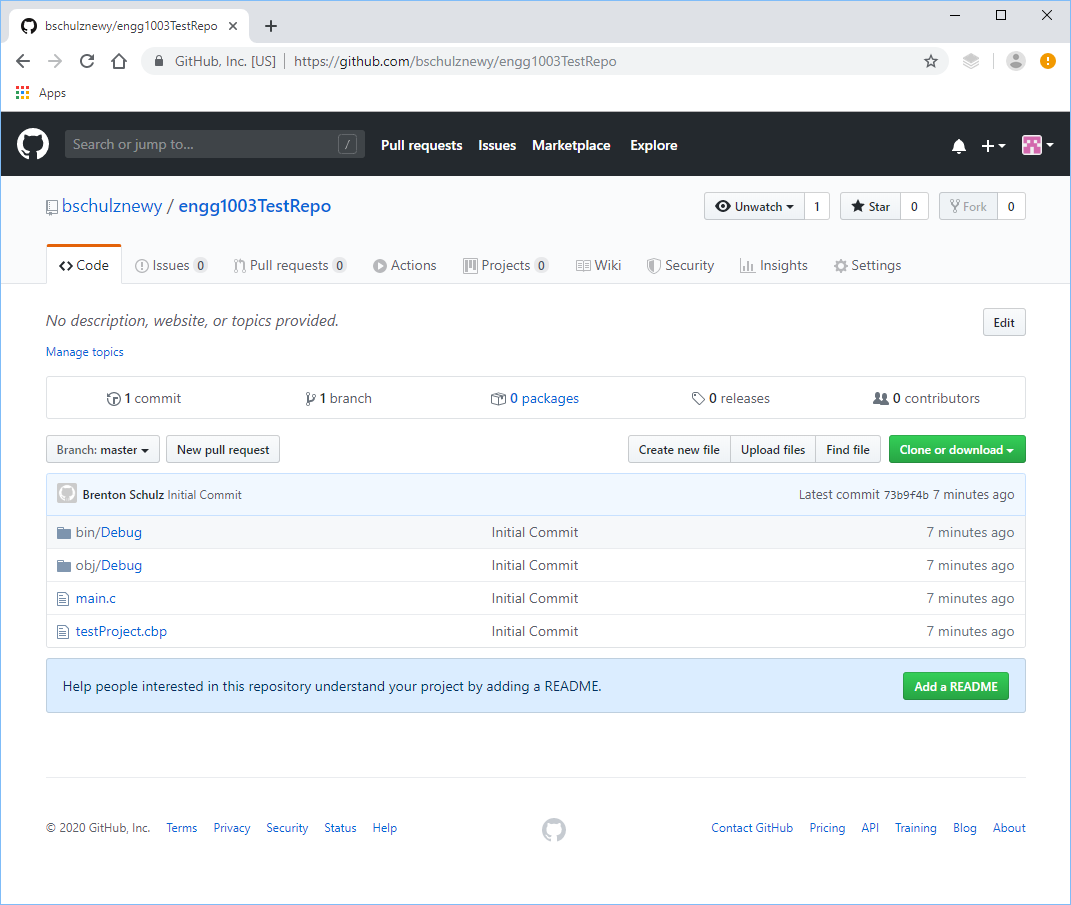
\includegraphics[width=0.9\textwidth]{Wk1Images/git10}
\end{center}
\end{figure}

\pagebreak
\item If you need to download (aka ``clone'') this repository on another machine you will need the URL provided by clicking the green ``Clone or download'' button:

\begin{figure}[H]
\begin{center}
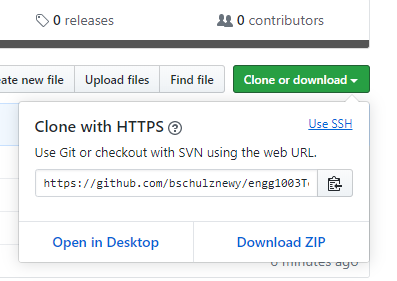
\includegraphics[width=0.7\textwidth]{Wk1Images/git11}
\end{center}
\end{figure}

\item On a different computer, or in a different folder on the same computer, go back to step 1 and re-open Git Gui through the right click context menu.

\item This time select ``Clone Existing Repository'' and follow the prompts to create a new copy of your lab 1 code.

\item If you make changes to the code you can open the Git GUI in the repository's top level folder and use the Git for Windows GUI to perform a ``stage'', followed by a ``commit'' (with an appropriate message) and, lastly, a ``push'' to upload new changes to your GitHub hosted repository.

\item The Git repository will keep track of any changes you make to your code. At any time you can view old versions and compare  what changed with each commit.

Make some changes to the code in Code::Blocks editor and perform a stage/commit/push and observe the changes on GitHub and in the Git GUI.

\end{enumerate}

\end{task}

\begin{task}{}{} Read more about how Git works and what it does here: \url{https://developer.ibm.com/tutorials/d-learn-workings-git/}. You probably won't understand everything, but that's not important right now. Just get some general exposure to the ideas and we'll fill in the practicalities later.
\end{task}

\pagebreak

\end{document}
